\section{Knowledge-Intensive Reasoning Tasks}
\label{sec:knowledge}
We begin with knowledge-intensive reasoning tasks like multi-hop question answering and fact verification.
As shown in Figure~\ref{fig:teaser}(1d), by interacting with a Wikipedia API, \model{} is able to retrieve information to support reasoning, while also use reasoning to target what to retrieve next, demonstrating a synergy of reasoning and acting.




\subsection{Setup}



\myparagraph{Domains} We consider two datasets challenging knowledge retrieval and reasoning: (1) HotPotQA~\citep{yang2018hotpotqa}, a multi-hop question answering benchmark that requires reasoning over two or more Wikipedia passages, and
(2) FEVER~\citep{thorne2018fever}, a fact verification benchmark where each claim is annotated SUPPORTS, REFUTES, or NOT ENOUGH INFO, based on if there exists a Wikipedia passage to verify the claim.
In this work, we operate in a question-only setup for both tasks, where models only receive the question/claim as input without access to support paragraphs, and have to rely on their internal knowledge or retrieve knowledge via interacting with an external environment to support reasoning.

\myparagraph{Action Space} We design a simple Wikipedia web API with three types of actions to support interactive information retrieval: 
(1) \textbf{\texttt{search}}[\texttt{entity}], which returns the first 5 sentences from the corresponding \texttt{entity} wiki page if it exists, or else suggests top-5 similar entities from the Wikipedia search engine, 
(2) \textbf{\texttt{lookup}}[\texttt{string}], which would return the next sentence in the page containing \texttt{string}, simulating Ctrl+F functionality on the browser. 
(3) \textbf{\texttt{finish}}[\texttt{answer}], which would finish the current task with \texttt{answer}.
We note that this action space mostly can only retrieve a small part of a passage based on exact passage name, which is significantly weaker than state-of-the-art lexical or neural retrievers. The purpose is to simulate how humans would interact with Wikipedia, and force models to retrieve via explicit reasoning in language.


\subsection{Methods}\label{sec:methods}

\myparagraph{\model{} Prompting} For HotpotQA and Fever, we randomly select 6 and 3 cases\footnote{We find more examples do not improve performance.} from the training set and manually compose \model{}-format trajectories to use as few-shot exemplars in the prompts. Similar to Figure~\ref{fig:teaser}(d), each trajectory consists of multiple thought-action-observation steps (i.e.\,dense thought), where free-form thoughts are used for various purposes.  {Specifically, we use a combination of thoughts that decompose questions (``I need to search x, find y, then find z''), extract information from Wikipedia observations (``x was started in 1844'', ``The paragraph does not tell x''), perform commonsense (``x is not y, so z must instead be...'') or arithmetic reasoning (``1844 < 1989''), guide search reformulation (``maybe I can search/look up x instead''), and synthesize the final answer (``...so the answer is x''). See Appendix~\ref{sec:prompts} for more details.}

\myparagraph{Baselines} We systematically ablate \model{}  trajectories to build prompts for multiple baselines (with formats as Figure~\ref{fig:teaser}(1a-1c)): 
(a) \textbf{Standard prompting} (\palm{}), which removes all thoughts, actions, observations in \model{} trajectories. 
(b) \textbf{Chain-of-thought prompting} (\reason{})~\citep{wei2022chain}, which removes actions and observations and serve as a reasoning-only baseline. We also build a self-consistency baseline (\reasons{})~\citep{wang2022self-consistency,wang2022rationale} by sampling 21 \reason{} trajectories with decoding temperature 0.7 during inference and adopting the majority answer, which is found to consistently boost performance over \reason{}. 
(c) \textbf{Acting-only prompt} (\act{}), which removes thoughts in \model{} trajectories, loosely resembling how WebGPT~\citep{nakano2021webgpt} interacts with the Internet to answer questions, though it operates on a different task and action space, and uses imitation and reinforcement learning instead of prompting.

\myparagraph{Combining Internal and External Knowledge} As will be detail in Section~\ref{subsec:results}, we observe that the problem solving process demonstrated by \model{} is more factual and grounded, whereas \reason{} is more accurate in formulating reasoning structure but can easily suffer from hallucinated facts or thoughts. We therefore propose to incorporate \model{}  and \reasons{}, and let the model decide when to switch to the other method based on the following heuristics:
    A) 
    \textbf{\model{} $\to$ \reasons{}}: when \model{} fails to return an answer within given steps, back off to \reasons{}. We set 7 and 5 steps for HotpotQA and FEVER respectively as we find more steps will not improve \model{} performance\footnote{{Of all trajectories with correct final answers, those with 7 steps on HotpotQA and 5 steps on FEVER only take up 0.84\% and 1.33\% respectively.}}. 
    B) 
    \textbf{  \reasons{} $\to$  \model{}}: when the majority answer among $n$ \reasons{} samples occurs less than $n/2$ times (i.e.\,internal knowledge might not support the task confidently), back off to \model{}. 


\myparagraph{Finetuning} Due to the challenge of manually annotating reasoning traces and actions at scale, we consider a bootstraping approach similar to \citet{zelikman2022star}, using 3,000 trajectories with correct answers generated by \model{} (also for other baselines) to finetune smaller language models (PaLM-8/62B) to decode trajectories (all thoughts, actions, observations) conditioned on input questions/claims. More details are in Appendix~\ref{sec:hotpot_finetune}.






\subsection{Results and Observations} \label{subsec:results}


\myparagraph{\model{} outperforms \act{} consistently} Table~\ref{table:reasoning} shows HotpotQA and Fever results using PaLM-540B as the base model with different prompting methods. 
We note that \model{} is better than \act{} on both tasks, demonstrating the value of reasoning to guide acting, especially for synthesizing the final answer, as shown in Figure~\ref{fig:teaser} (1c-d). Fine-tuning results~\ref{fig:finetune} also confirm the benefit of reasoning traces for more informed acting.

\begin{table}[t]
\begin{minipage}{.42\linewidth}
    \centering


\resizebox{\columnwidth}{!}{%
\begin{tabular}{l|c|c}
\toprule
    \multirow{2}{*}{\textbf{Prompt Method\footnote{\tiny HotpotQA EM is 27.1, 28.9, 33.8 for \palm{}, \reason{}, \reasons{} in \cite{wang2022rationale}.}}} & \textbf{HotpotQA} & \textbf{Fever}  \\
    & (EM) & (Acc) \\ 
\midrule
    \palm{}  & 28.7 & 57.1 \\
    \reason{}{\scriptsize~\citep{wei2022chain}} & 29.4 & 56.3 \\ 
    \reasons{}{\scriptsize~\citep{wang2022self-consistency}} & 33.4 & 60.4 \\
    \midrule
    \act  & 25.7 & 58.9 \\ 
    \model   & 27.4 & {60.9} \\
    \reasons{} $\to$ \model   & 34.2 & \textbf{64.6} \\
    \model $\to$ \reasons{} & \textbf{35.1} & 62.0 \\ \midrule \midrule
    \textbf{Supervised SoTA\footnote{\tiny\citep{zhu2021adaptive,lewis2020retrieval}}} & 67.5 & 89.5 \\

    
\bottomrule
\end{tabular}%
}
\caption{
PaLM-540B prompting results on HotpotQA and Fever. 
}
\label{table:reasoning}


\end{minipage}%
\hspace{5pt}
\begin{minipage}{.57\linewidth}
    \centering
    
    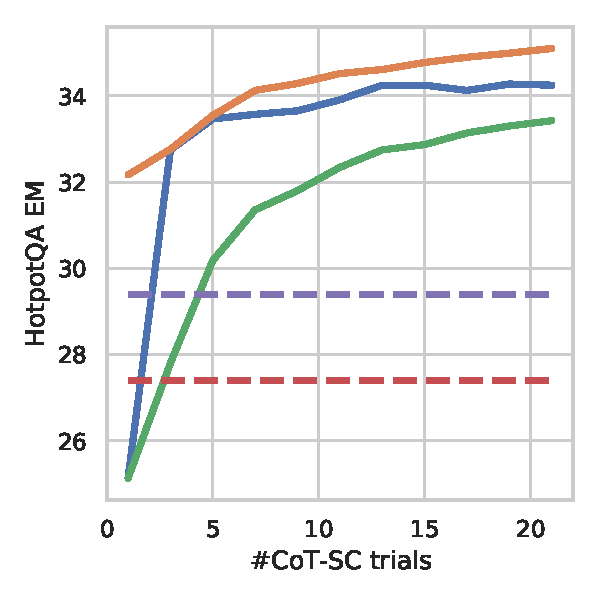
\includegraphics[width=.49\textwidth]{iclr2023/figure/cots_scale.pdf}
    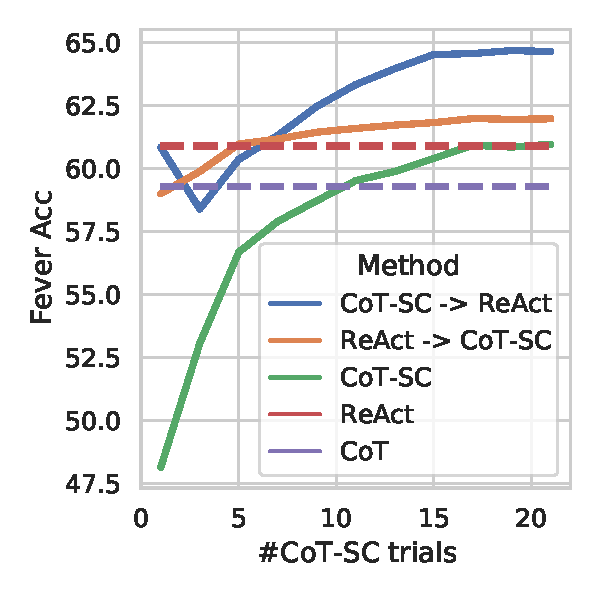
\includegraphics[width=.49\textwidth]{iclr2023/figure/fever_cots_scale.pdf}
    \captionof{figure}{PaLM-540B prompting results with respect to number of \reasons{} samples used.}
    \label{fig:cots_to_react}
    
    


\end{minipage}%
\vspace{-10pt}
\end{table}



\begin{table}[t]
\scriptsize
\begin{minipage}{1.0\linewidth}
    \centering
\begin{tabular}{l|clll}
\toprule
    & Type & Definition & \model & \reason \\
\midrule
\multirow{2}{*}{Success} & True positive & Correct reasoning trace and facts & 94\% & 86\% \\ & False positive & Hallucinated reasoning trace or facts & 6\% & 14\%\\
    \hline
    \multirow{4}{*}{Failure} & Reasoning error & Wrong reasoning trace (including failing to recover from repetitive steps) & 47\% & 16\% \\ & Search result error & Search return empty or does not contain useful information & 23\% & - \\ & Hallucination & Hallucinated reasoning trace or facts & 0\% & 56\% \\ & Label ambiguity & Right prediction but did not match the label precisely & 29\% & 28\%\\
\bottomrule
\end{tabular}
\caption{
Types of success and failure modes of \model{} and \reason{} on HotpotQA, as well as their percentages in randomly selected examples studied by human. %
}
\label{table:human_study_categories}
\end{minipage}%
\vspace{-10pt}
\end{table}



\myparagraph{\model{} vs. \reason{}} 
On the other hand, \model{} outperforms \reason{} on Fever (60.9 vs.\,56.3) and slightly lags behind \reason{} on HotpotQA (27.4 vs.\,29.4). 
Fever claims for SUPPORTS/REFUTES might only differ by a slight amount (see Appendix~\ref{sec:fever_trajs}), so acting to retrieve accurate and up-to-date knowledge is vital. 
To better understand the behavioral difference between \model{} and \reason{} on HotpotQA, we randomly sampled 50 trajectories with correct and incorrect answers (judged by EM) from \model{} and \reason{} respectively (thus 200 examples in total), and manually labeled their success and failure modes in Table~\ref{table:human_study_categories}. 
Some key observations are as follows:

\quad A) \textbf{Hallucination is a serious problem for \reason}, resulting in much higher false positive rate than \model{} (14\% vs. 6\%) in success mode, and make up its major failure mode (56\%).
In contrast, the problem solving trajectory of \model is more grounded, fact-driven, and trustworthy, thanks to the access of an external knowledge base.

\quad B) \textbf{While interleaving reasoning, action and observation steps improves \model's groundedness and trustworthiness, such a structural constraint also reduces its flexibility in formulating reasoning steps}, leading to more reasoning error rate than \reason. 
we note that there is one frequent error pattern specific to \model, in which the model repetitively generates the previous thoughts and actions, and we categorize it as part of ``reasoning error'' as the model fails to reason about what the proper next action to take and jump out of the loop\footnote{We suspect that this could be due to the sub-optimal greedy decoding procedure, and future work using better decoding (e.g.\,beam search) might help address this issue.}. 

\quad C) \textbf{For \model, successfully retrieving informative knowledge via search is critical.} Non-informative search, which counts for 23\% of the error cases, derails the model reasoning and gives it a hard time to recover and reformulate thoughts. This is perhaps an expected trade-off between factuality and flexibility, which motivates our proposed strategies of combining two methods.


We provide examples for each success and failure modes in Appendix \ref{sec:human_study_examples}. We also find some HotpotQA questions may contain outdated answer labels, see Figure~\ref{fig:date} for example.

\myparagraph{\model{} + \reason{}-SC perform best for prompting LLMs} Also shown in Table~\ref{table:reasoning}, the best prompting method on HotpotQA and Fever are \model{} $\to$ \reasons{} and \reasons{}  $\to$  \model{} respectively. Furthermore, Figure~\ref{fig:cots_to_react} shows how different methods perform with respect to the number of \reasons{} samples used. While two \model{} + \reasons{} methods are advantageous at one task each, they both significantly and consistently outperform \reasons{} across different number of samples, reaching \reasons{} performance with 21 samples using merely 3-5 samples. These results indicate the value of properly combining model internal knowledge and external knowledge for reasoning tasks. 

\begin{figure}[t]
    \centering
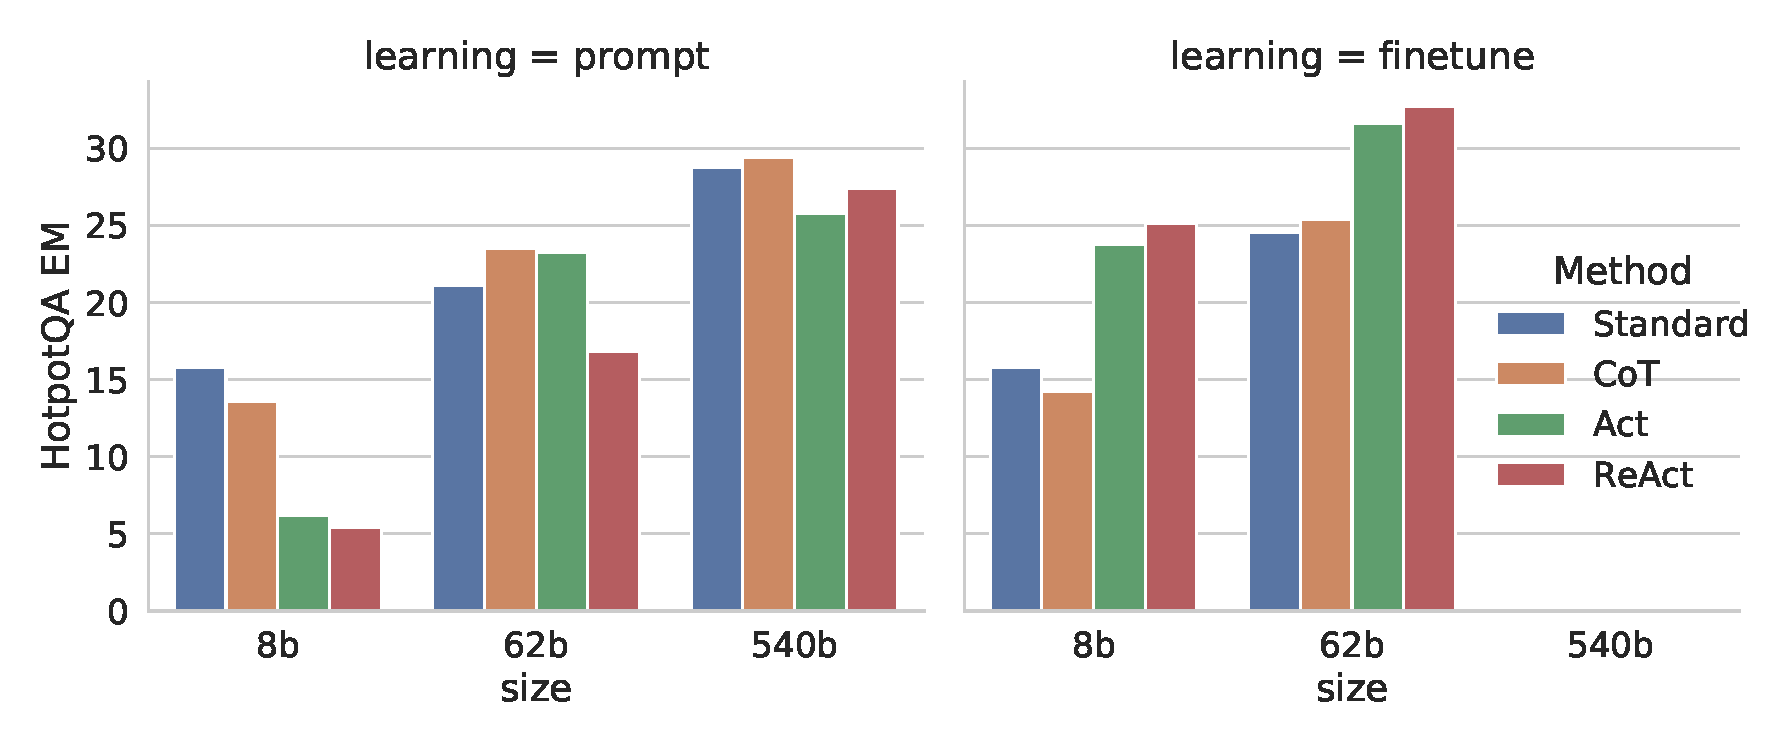
\includegraphics[width=.76\textwidth]{iclr2023/figure/hotpot_finetune.pdf}
\vspace{-5pt}
    \caption{Scaling results for prompting and finetuning on HotPotQA with \model{} (ours) and  baselines.}
    \label{fig:finetune}
    \vspace{-12pt}
\end{figure}



\myparagraph{\model{} performs best for fine-tuning} Figure~\ref{fig:finetune} shows the scaling effect of prompting/finetuning four methods (\palm{}, \reason{}, \act{}, \model{}) on HotpotQA. With PaLM-8/62B, prompting \model{} performs worst among four methods due to the difficulty to learn both reasoning and acting from in-context examples. However, when finetuned with just 3,000 examples, \model{} becomes the best method among the four, with PaLM-8B finetuned \model{} outperforming all PaLM-62B prompting methods, and PaLM-62B finetuned \model{} outperforming all 540B prompting methods. In contrast, finetuning \palm{} or \reason{} is significantly worse than finetuning \model{} or \act{} for both PaLM-8/62B, as the former essentially teaches models to memorize (potentially halluincated) knowledge facts, and the latter teaches models how to (reason and) act to access information from Wikipedia, a more generalizable skill for knowledge reasoning. 
As all prompting methods are still significantly far from domain-specific state-of-the-art approaches (Table~\ref{table:reasoning}), we believe finetuning with more human-written data might be a better way to unleash the power of \model{}. 





